\documentclass[hyperref={pdfpagelayout=SinglePage}]{beamer}

%Template
\usetheme{Warsaw}
\usecolortheme{default}
\usefonttheme[onlymath]{serif}

%Packages
\usepackage[utf8]{inputenc}
\usepackage[spanish,activeacute]{babel}
\usepackage{lipsum}
\usepackage{graphicx}
\usepackage{fancyhdr}
\usepackage{float}
\usepackage{adjustbox}
\usepackage{subfigure}
\usepackage{amsmath}
\usepackage{ragged2e}
\usepackage{color}
\usepackage{listings}
\usepackage{animate}
\usepackage{hyperref}

%Code
\lstset{ %
basicstyle=\small,       % the size of the fonts that are used for the code
numbers=none,                   % where to put the line-numbers
numberstyle=\footnotesize,      % the size of the fonts that are used for the line-numbers
stepnumber=1,                   % the step between two line-numbers. If it is 1 each line will be numbered
numbersep=5pt,                  % how far the line-numbers are from the code
backgroundcolor=\color{white},  % choose the background color. You must add \usepackage{color}
showspaces=false,               % show spaces adding particular underscores
showstringspaces=false,         % underline spaces within strings
showtabs=false,                 % show tabs within strings adding particular underscores
frame=single,           % adds a frame around the code
tabsize=4,          % sets default tabsize to N spaces
captionpos=b,           % sets the caption-position to bottom
breaklines=true,        % sets automatic line breaking
breakatwhitespace=false,    % sets if automatic breaks should only happen at whitespace
escapeinside={\%*}{*)}          % if you want to add a comment within your code
}

%Captions
\renewcommand{\lstlistingname}{Código}
\renewcommand\spanishtablename{Tabla}
\renewcommand{\figurename}{Gráfico}

%More
\makeatletter
\@addtoreset{subfigure}{framenumber}
\makeatother

\expandafter\def\expandafter\insertshorttitle\expandafter{%
  \insertshorttitle\hfill%
  \insertframenumber\,/\,\inserttotalframenumber}

\newcommand\Wider[2][5em]{%
\makebox[\linewidth][c]{%
  \begin{minipage}{\dimexpr\textwidth+#1\relax}
  \raggedright#2
  \end{minipage}%
  }%
}

%List of parts
\makeatletter
\AtBeginPart{%
    \addtocontents{parttoc}{\protect\beamer@partintoc{\the\c@part}{\beamer@partnameshort}{\the\c@page}}%
    \frame{\partpage}%
}
\newcommand{\parttableofcontents}{\@starttoc{parttoc}}
\newcommand{\beamer@partintoc}[3]{#2\par}
\makeatother

%Document Data
\title{Dinámica Molecular regida por el paso temporal}
\subtitle{Trabajo Práctico Nro. 4}
\author{Badi Leonel, Buchhalter Nicolás Demián y Meola Franco Román}
\subject{Simulación de Sistemas}
\date{\today}

\begin{document}

\begin{frame}
    \frametitle{} 
    \titlepage
    \centering
	Grupo 3
\end{frame}

\begin{frame}
\frametitle{Fundamentos}
\framesubtitle{Introducción}
\begin{itemize}
	\item Vamos a comparar los errores cometidos por distintos sistemas de integración
	\item Oscilador amortiguado: Sistema con sólo una partícula puntual cuya solución analítica es conocida
	\item Se implementaron:
	\begin{itemize}
		\item \textit{Beeman}
		\item \textit{Velocity Verlet}
		\item \textit{Gear Predictor Corrector de orden 5}
	\end{itemize}
\end{itemize}
\end{frame}

\subsection{Variables relevantes}

\begin{frame}
\frametitle{Fundamentos}
\framesubtitle{Variables relevantes}
\begin{itemize}
\item \textbf{Parámetros del oscilador}
	\begin{itemize}
		\item $m = 70$
		\item $k = 10000$
		\item $\gamma = 100$
		\item $t_{f} = 5$ 
	\end{itemize}
\item \textbf{Condiciones iniciales del oscilador}
	\begin{itemize}
		\item $r_{0} = 1$
		\item $v_{0} = -\frac{2\gamma}{m}$
	\end{itemize}
\end{itemize}
\end{frame}

\section{Implementación}

\subsection{Simulación}

\begin{frame}[fragile]
\frametitle{Implementación}
\framesubtitle{Cálculo Numérico}
\begin{lstlisting}[language=Java, caption = Método de Gear Predictor Corrector]
void simulateGear(double time, double deltaT) {
	double simTime = 0;
    Oscilator oscilator = new Oscilator();
	oscilator.writePositionAndError();
    oscilator.makeEulerStep(deltaT);
    simTime += deltaT;
	oscilator.writePositionAndError();
    while (simTime < time) {
    	oscilator.makeGearStep(deltaT);
        simTime += deltaT;
		oscilator.writePositionAndError();
    }
}
\end{lstlisting}
\end{frame}

\begin{frame}
\frametitle{Implementación}
\framesubtitle{Detalles de precisión}
\begin{itemize}
	\item Todas las operaciones se realizan en \texttt{double}
	\item Se utilizan cinco cifras decimales como \texttt{output} en los archivos de salida de resultados y errores
\end{itemize}
\end{frame}

\section{Resultados}

\subsection{Tablas}

\begin{frame}
\frametitle{Resultados}
\framesubtitle{Error total normalizado por el número total de pasos para distintos valores de $\Delta t$}
\begin{center}
\begin{table}[h]
\centering
\adjustbox{max height=\dimexpr\textheight-3.0cm\relax,
           max width=\textwidth}{
\begin{tabular}{ccc}
\hline
\textbf{$\Delta t$} & \textbf{Método} & \textbf{$E$}\\ \hline
0.01&\textit{Beeman}&0,00471\\
0.01&\textit{Verlet}&0,00663\\
0.01&\textit{Gear}&0,33624\\
0.001&\textit{Beeman}&0,00235\\
0.001&\textit{Verlet}&0,00225\\
\textbf{0.001}&\textbf{\textit{Gear}}&\textbf{-0,00199}\\
0.0001&\textit{Beeman}&0,00225\\
0.0001&\textit{Verlet}&0,00224\\
0.0001&\textit{Gear}&0,00228\\
\end{tabular}
}
\caption{Suma de las diferencias al cuadrado para todos los pasos temporales normalizado por el número total de pasos}
\end{table}
\end{center}
\end{frame}

\subsection{Gráficos}

\begin{frame}
\Wider{
\frametitle{Resultados}
\framesubtitle{Gráfico de $x(t)$ para el oscilador puntual amortiguado con $\Delta t = 0.01$}
\begin{figure}[H]
        \centering
        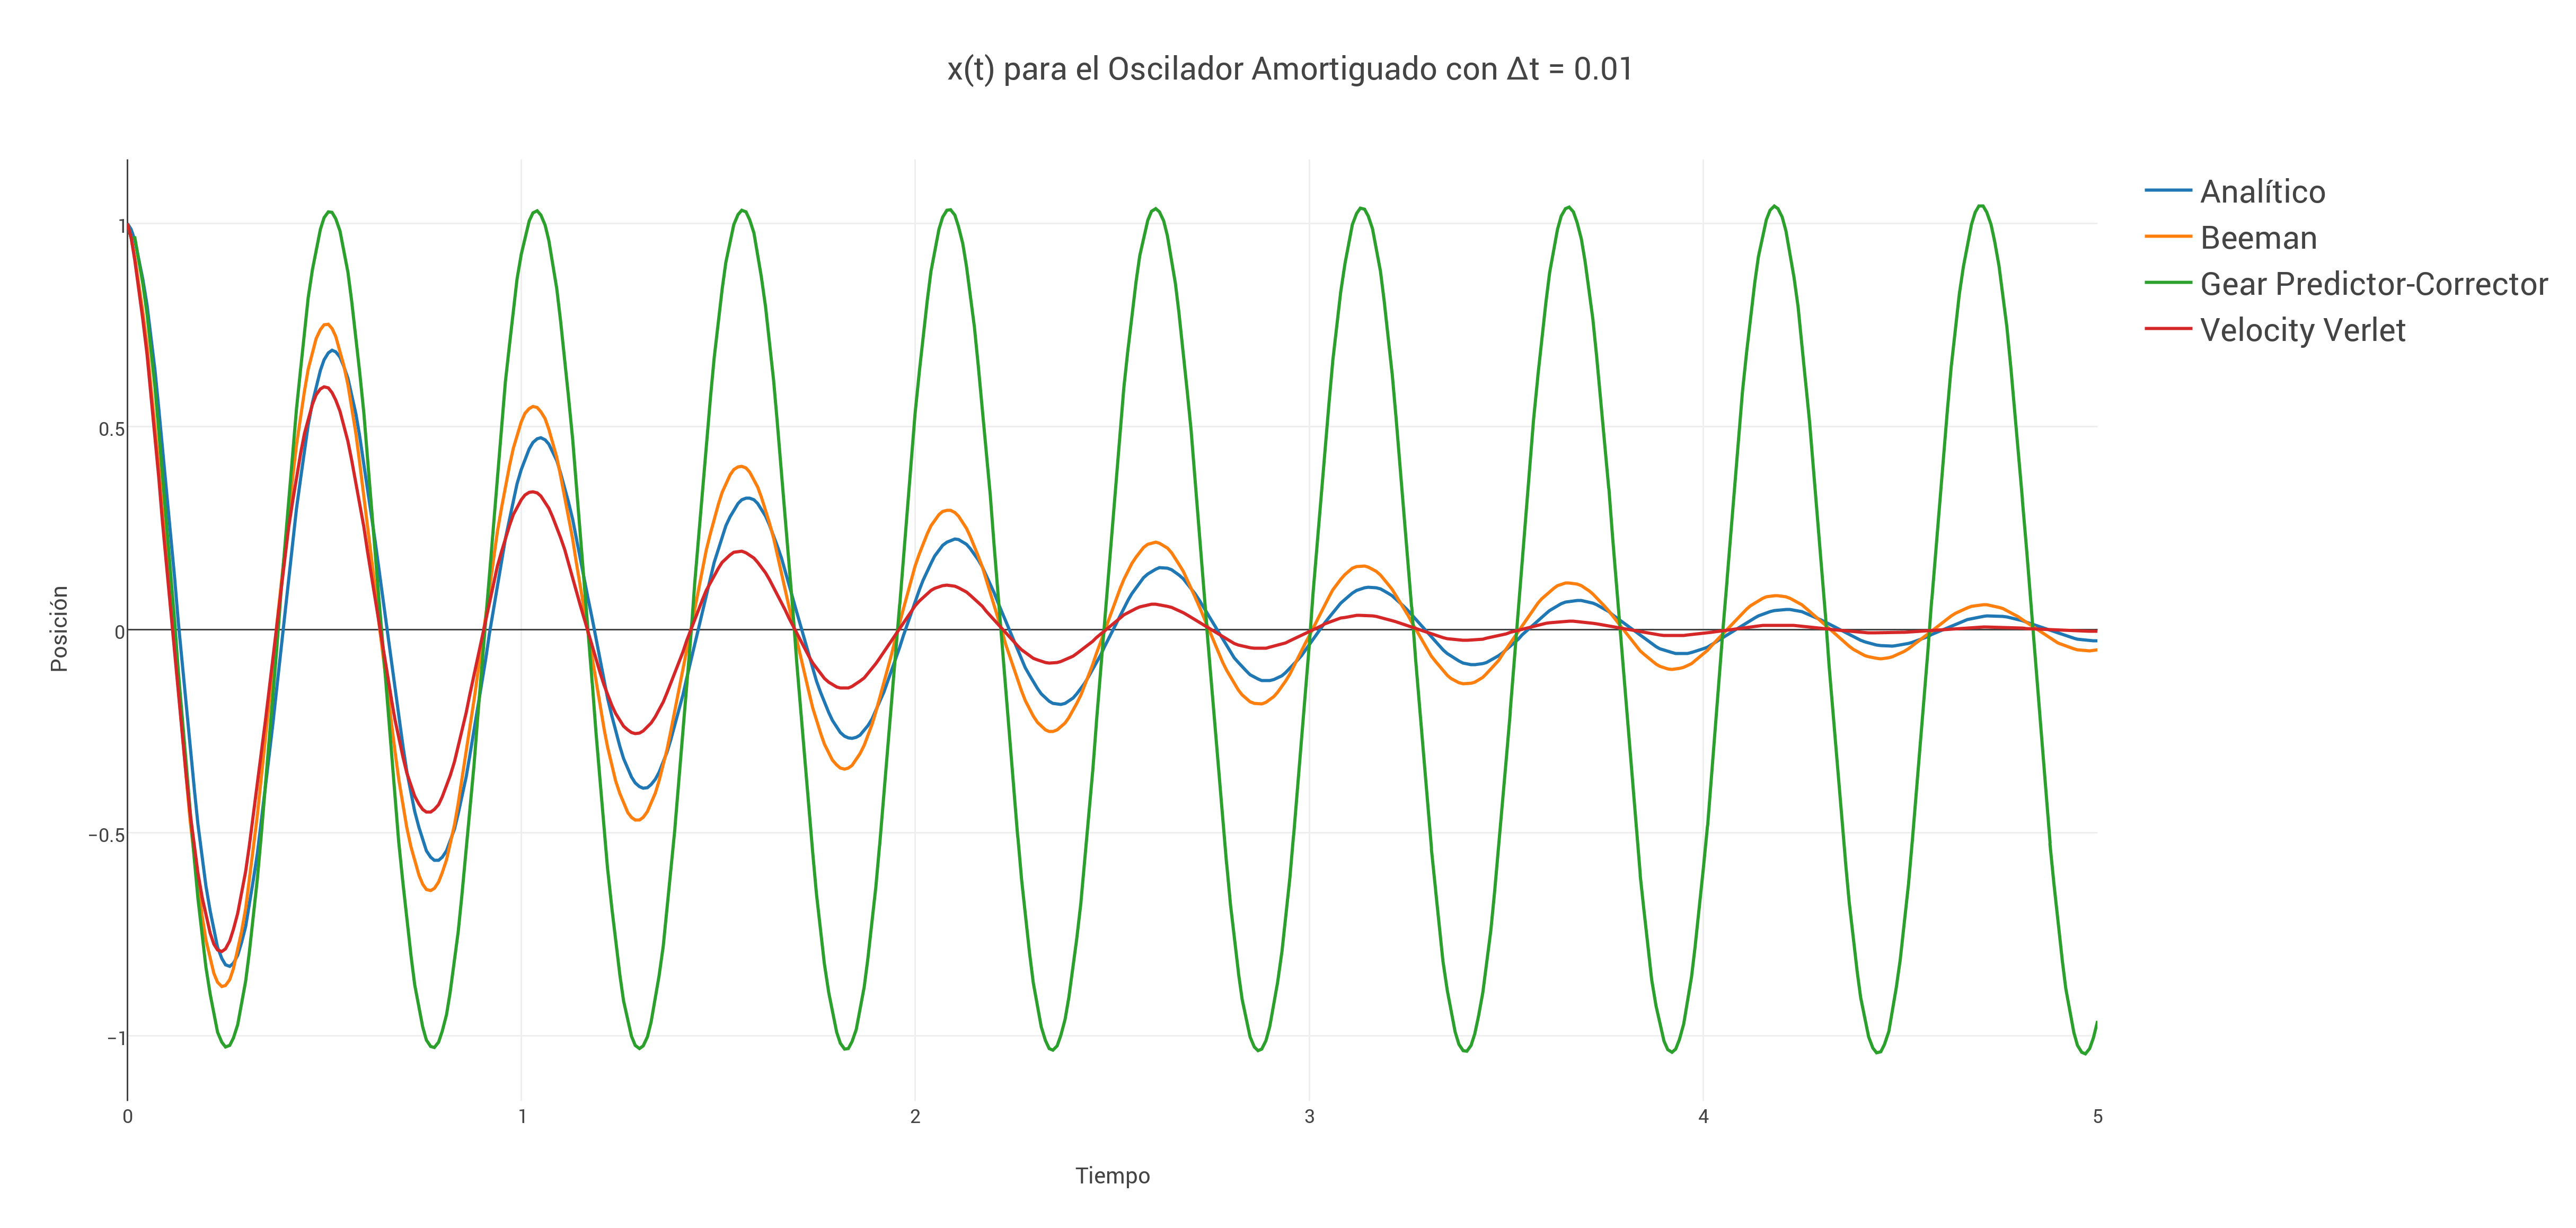
\includegraphics[width=\textwidth]{{images/0.01}.png}
\end{figure}
}
\end{frame}

\begin{frame}
\Wider{
\frametitle{Resultados}
\framesubtitle{Gráfico de $x(t)$ para el oscilador puntual amortiguado con $\Delta t = 0.001$}
\begin{figure}[H]
        \centering
        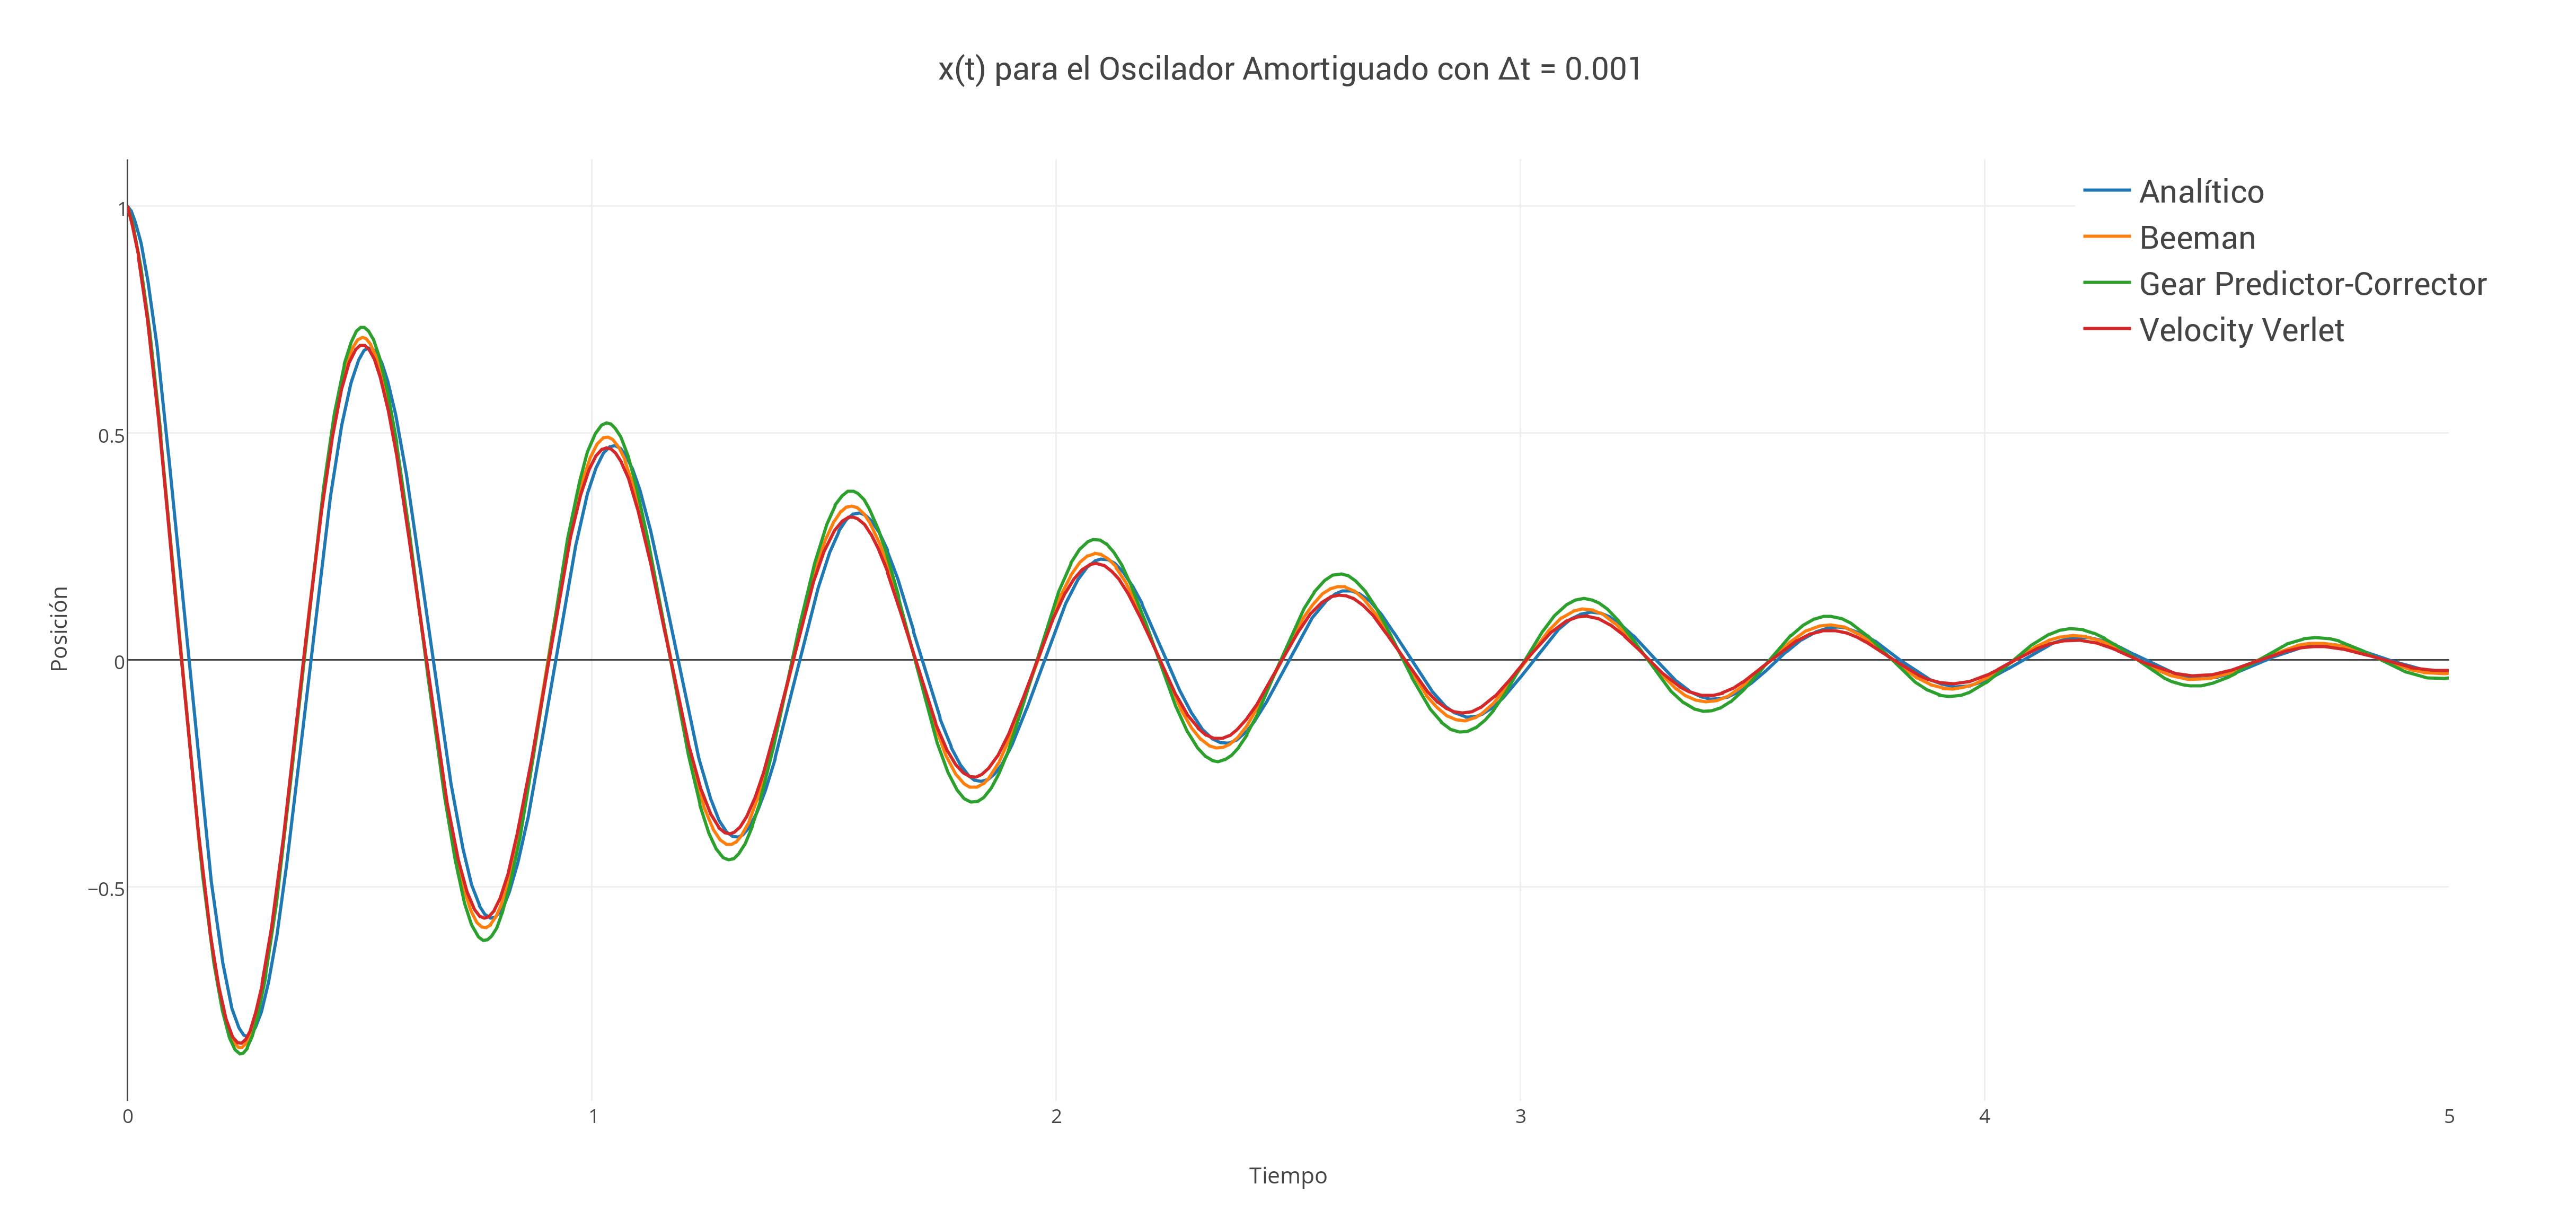
\includegraphics[width=\textwidth]{{images/0.001}.png}
\end{figure}
}
\end{frame}

\begin{frame}
\Wider{
\frametitle{Resultados}
\framesubtitle{Gráfico de $E$ para el oscilador puntual amortiguado con $\Delta t = 0.01$}
\begin{figure}[H]
        \centering
        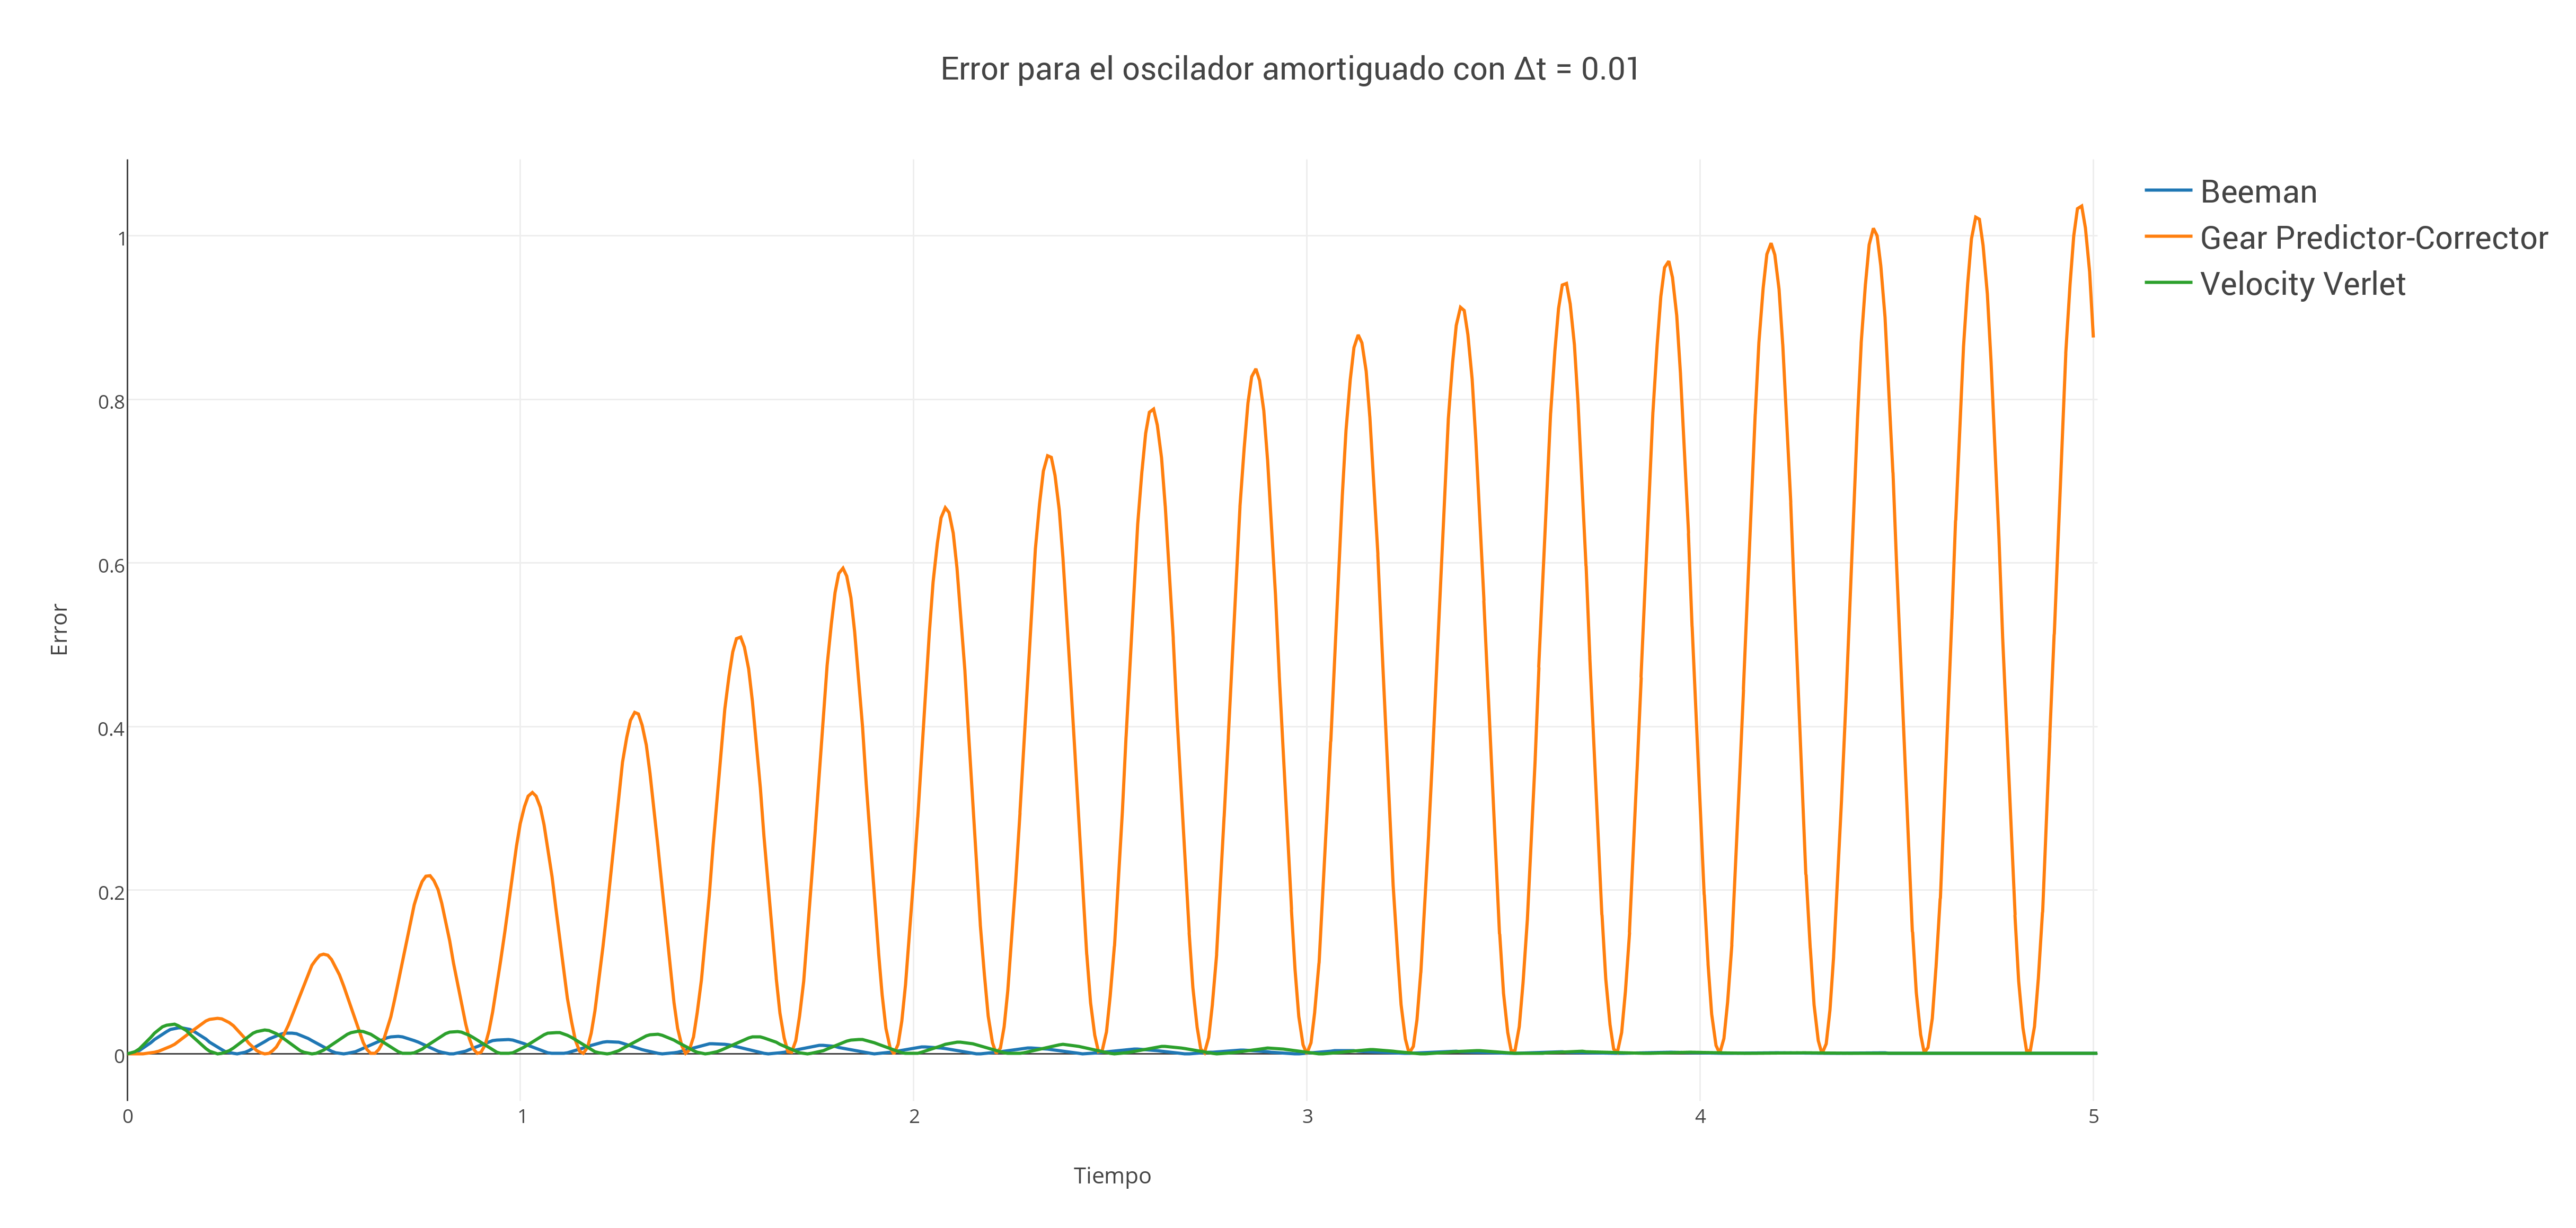
\includegraphics[width=\textwidth]{{images/Error-0.01}.png}
\end{figure}
}
\end{frame}

\begin{frame}
\Wider{
\frametitle{Resultados}
\framesubtitle{Gráfico de $E$ para el oscilador puntual amortiguado con $\Delta t = 0.001$}
\begin{figure}[H]
        \centering
        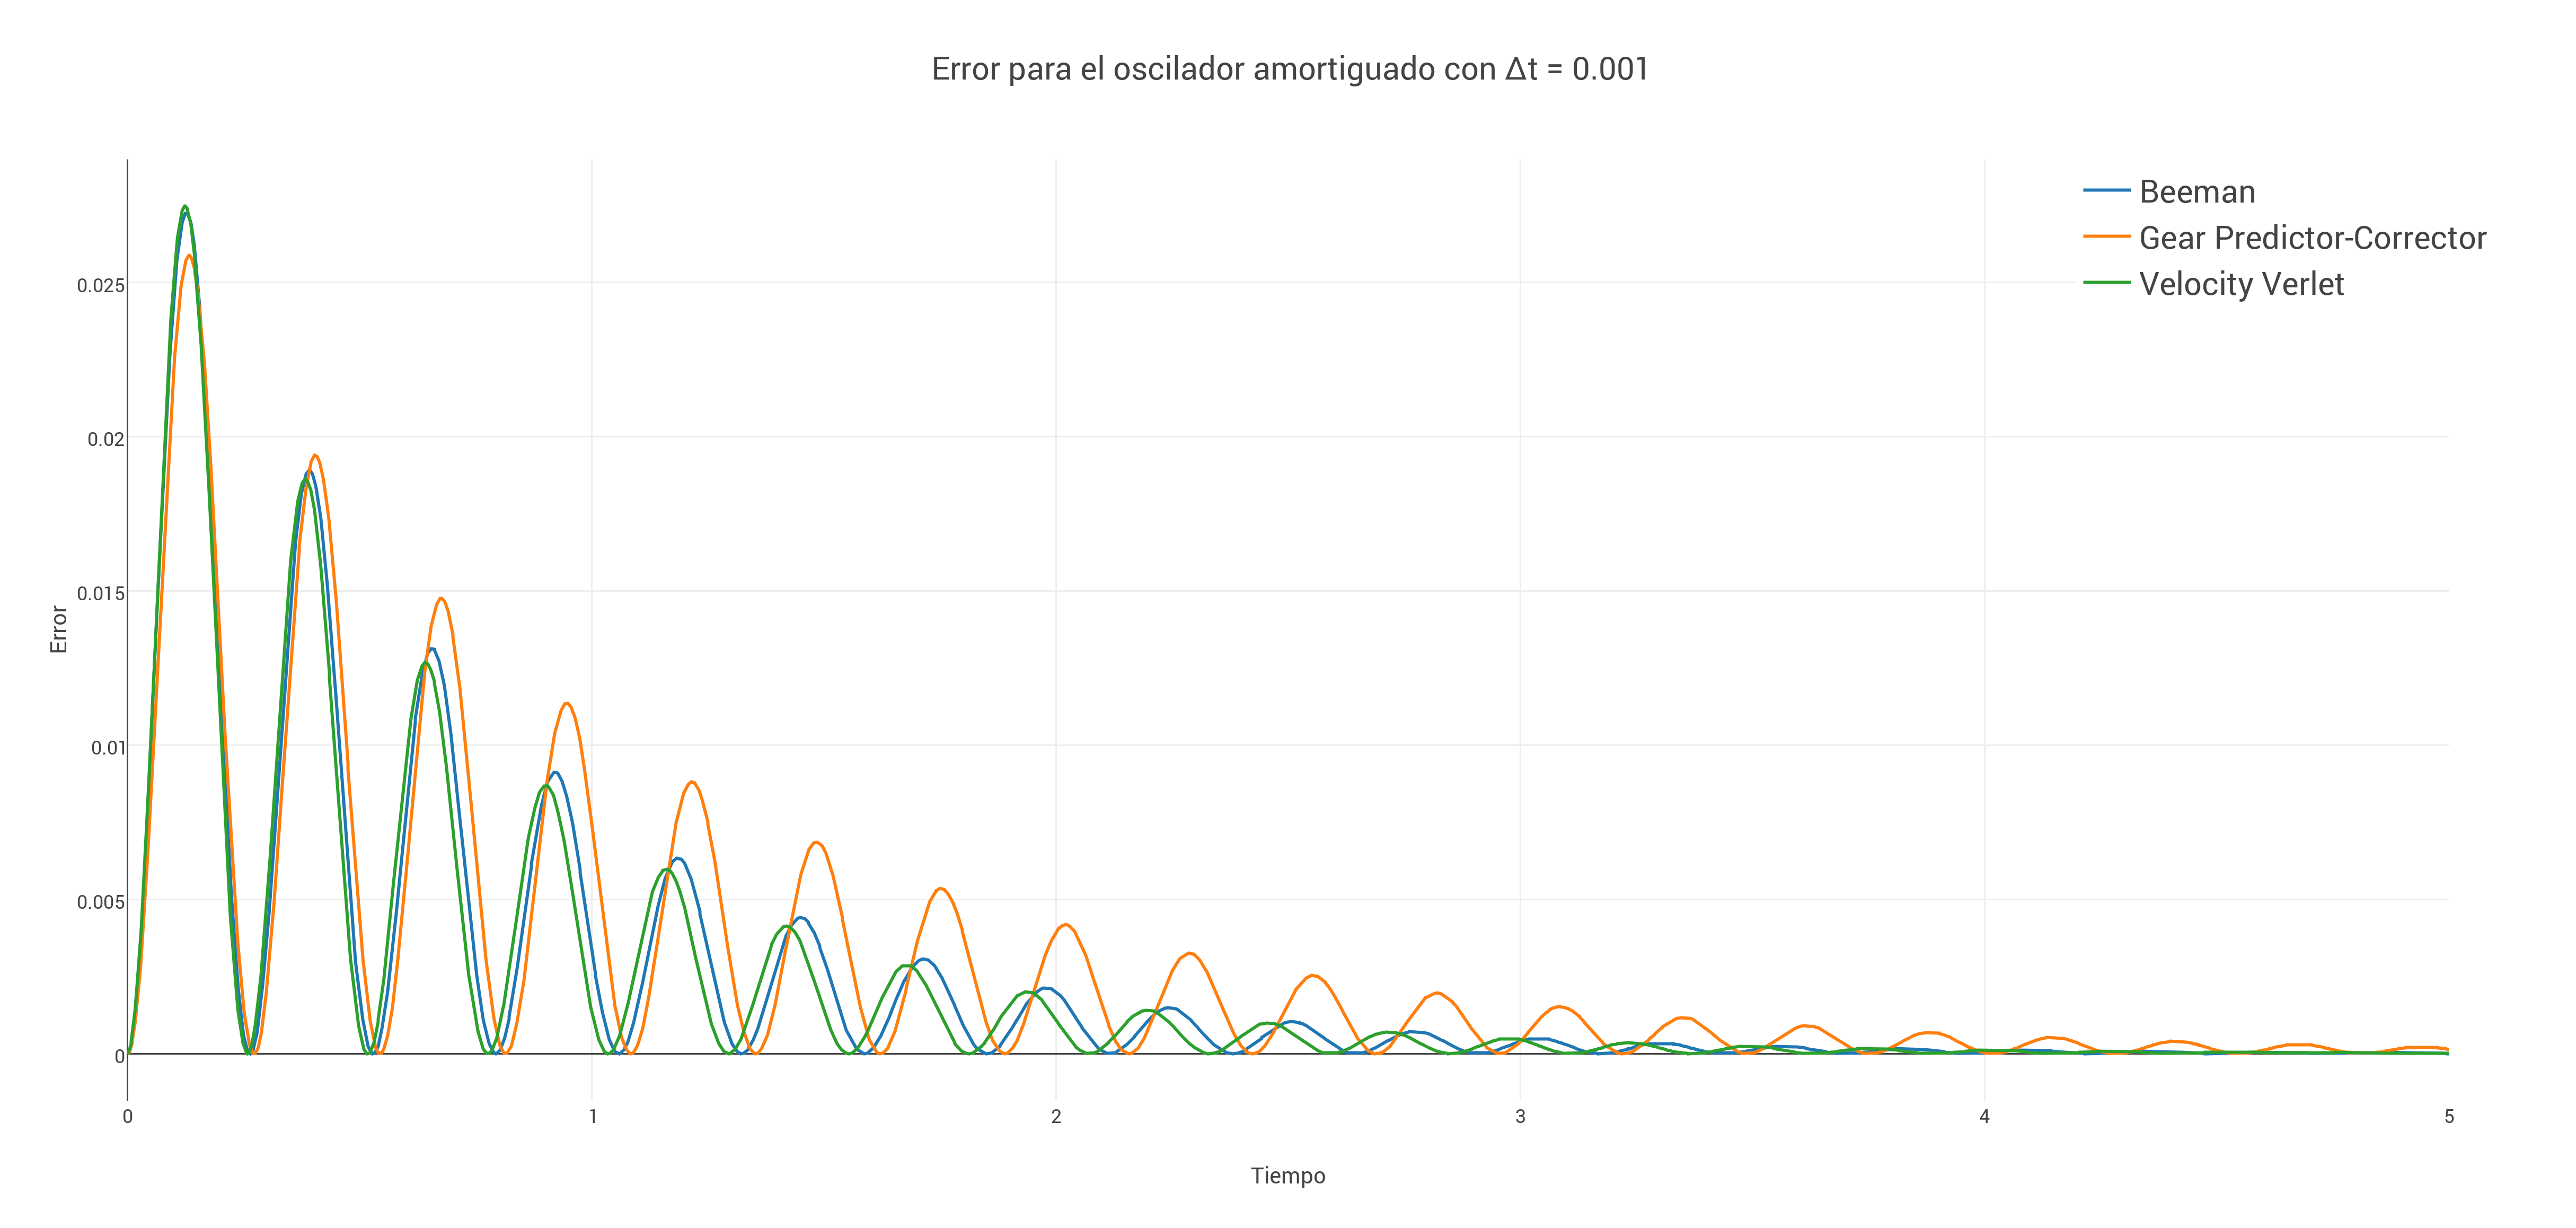
\includegraphics[width=\textwidth]{{images/Error-0.001}.png}
\end{figure}
}
\end{frame}

\subsection{Conclusiones}

\begin{frame}
\frametitle{Conclusiones}
\begin{itemize}
	\item Para una cantidad de pasos baja (500 pasos, $\Delta t = 0.01$), el error de \textit{Gear Predictor-Corrector} aumenta, simulando un oscilador no amortiguado
	\item Con un $\Delta t = 0.001$ obtuvimos resultados con errores muy bajos para los tres métodos
	\item Con 50000 pasos ($\Delta t = 0.0001$), los tres métodos tienen un error que varía recíen en la quinta cifra decimal
	\item El esquema de integración que mejor resulta para este sistema es \textit{Gear Predictor-Corrector} para $\Delta t = 0.001$, es decir, 5000 pasos
	\end{itemize}	
\end{frame}
    
\part{Formación del Sistema Solar}
    
\section{Fundamentos}

\subsection{Introducción}

\begin{frame}
\frametitle{Fundamentos}
\framesubtitle{Introducción}
\begin{itemize}
	\item Usando el esquema de integración de \textit{Beeman} vamos a simular el nacimiento del sistema solar
	\item Se simularán $N$ partículas que orbitan alrededor del Sol
	\item Las partículas se irán agrupando en planetas a medida que el sistema evolucione
\end{itemize}
\end{frame}

\subsection{Variables relevantes}

\section{Implementación}

\subsection{Generación de los agentes}

\begin{frame}
\frametitle{Implementación}
\framesubtitle{Generación de los agentes}
\begin{itemize}
	\item Posiciones $(x,y)$ aleatorias para todas las partículas
	\item $v_{t_0}$ tal que todas las partículas tengan el mismo $L$
	\item $v_{n_0} = 0$
	\item Distancia al sol entre $1 \times 10^{9}$
 y $1 \times 10^{10}$
	\item Ángulo respecto al Sol $\epsilon$  $[0, 2 \pi]$
\end{itemize}
\end{frame}

\subsection{Simulación}

\begin{frame}
\frametitle{Simulación}
\framesubtitle{Variables relevantes}
\begin{itemize}
	\item $\Delta t$: cantidad de pasos
	\item $k$: relación entre cantidad de pasos simulados y visualizados.
	\item \texttt{time}: Tiempo en segundos a visualizar
\end{itemize}
\end{frame}

\begin{frame}
\frametitle{Simulación}
\framesubtitle{Detalles de implementación}
\begin{itemize}
	\item Utilizamos el \textit{Cell Index Method} para calcular las colisiones de las partículas
	%TODO 
	%\item Se modificó el \textit{Cell Index Method} para que soporte radios de interacción distintos para cada una de las partículas
	\item Para las partículas que se alejen más de $2 \times 10^{4}$ del centro, no las consideramos dentro del sistema
	\item En colisión de particulas, se mantiene el momento angular pero la velocidad normal resultante se resuelve como un choque perfectamente inelastico.
	\begin{itemize}
		\item Por lo tanto la energia en el sistema no se conserva ya que se disipa como energia interna dentro de las particulas.
		\item Se conserva solamente la energia orbital.
	\end{itemize}
\end{itemize}
\end{frame}

\begin{frame}
\frametitle{Simulación}
\framesubtitle{Problemas encontrados}
\begin{itemize}
	\item \textbf{Tratamiento de números de grandes dimensiones}
	\begin{itemize}
		\item Necesitamos poder mantener en memoria números grandes utilizando la precisión \texttt{double}
		\item Se normalizó $r$ a $1 \times 10^{6}$
		\item Se normalizó $m$ a $2 \times 10^{25}$
		\item Se modifico la constante G.
	\end{itemize}
	\item \textbf{El radio de las partículas es muy chico en comparación con las dimensiones del sistema solar}
	\begin{itemize}
			\item Esto dificulta la visualización, sobre todo para una gran cantidad de partículas
			\item El $r_{c}$ es distinto al $r_{v}$ (radio de visualización)
	\end{itemize}
\end{itemize}
\end{frame}

\begin{frame}[fragile]
\frametitle{Implementación}
\framesubtitle{Simulación}
\begin{lstlisting}[language=Java, caption = Simulación]
void simulate(int k, double dt, int time){
	write();
	moveEuler(dt);
	int framesWrited = 1;
	double totalTimeSimulated = dt;
	while(totalTimeSimulated < time) {
 		for(int i=0; i<k; i++) {
			moveBeeman(dt);
			findNeighbours();
			collidePlanets();
            totalTimeSimulated += dt;
			write();
		}
		write();
		framesWrited++;
    }
}
\end{lstlisting}
\end{frame}

\subsection{Visualización}

\begin{frame}
\frametitle{Implementación}
\framesubtitle{Visualización}
\begin{itemize}
	\item La simulación y la visualización son independientes
	\item El algoritmo de simulación escribe un archivo \texttt{.tsv} con los siguientes datos:
\begin{itemize}
\item $(x,y)$
\item $r$
\item Color RGB para indicar la masa de la particula, cuanto mayor masa mas blanca la particula\end{itemize}
\item Se generan particulas temporales para visualizar los choques.
\item Por último, se carga en \texttt{Ovito} el archivo de salida\texttt{.tsv} para realizar la visualización
\end{itemize}
\end{frame}


\section{Resultados}

\subsection{Animaciones}

\begin{frame}
\frametitle{Resultados}
\framesubtitle{Animación de la simulación para $N = 100$}
\begin{figure}[H]
	\centering
	\animategraphics[loop,controls,width=0.75\textheight]{10}{animation/100eliptica}{0000}{0200}
\end{figure}
\end{frame}

\begin{frame}
\frametitle{Resultados}
\framesubtitle{Animación de la simulación para $N = 1000$}
\begin{figure}[H]
	\centering
	\href{https://youtu.be/hILxOjPESgA}{Link al video}
\end{figure}
\end{frame}

\begin{frame}
\frametitle{Resultados}
\framesubtitle{Animación de la simulación para $N = 10000$}
\begin{figure}[H]
	\centering
	\href{https://youtu.be/hILxOjPESgA}{Link al video}
\end{figure}
\end{frame}

\subsection{Conclusiones}

\begin{frame}
\frametitle{Conclusiones}
\begin{itemize}
	\item El paso temporal ($\Delta t$) se podria ir variando si calculamos la cota de la velocidad.
	\item Metodo ineficiente en el caso de tener tiempos de vuelos altos.
	\item Para calcular el paso temporal ($\Delta t$) hay que considerar el error de aproximacion deseado, asi como el ($\Delta t$) para que no se omitan eventos.
	\end{itemize}	
\end{frame}

\begin{frame}[plain,c]
\begin{center}
	\Huge Gracias
\end{center}
\end{frame}
    
\end{document}
